
\documentclass[12pt, oneside]{extbook} % the document type needs to be change
\usepackage{geometry}
\usepackage{listings}
\usepackage{graphicx}
\usepackage[utf8]{inputenc}
\usepackage[T1]{fontenc}
\usepackage[italian]{babel}

\geometry{
    top = 1.5cm,
    bottom = 1.5cm,
    left = 2cm,
    right=2cm,
}

\begin{document}

\chapter*{BGP}

\section{Introduzione}
Parliamo di BGP perché è uno dei building blocks fondamentali di Internet, vediamo BGP non in dettaglio ma sulla parte di sicurezza.
\\Dopo aver capito come funziona BGP vederemo MPLS e delle VPNs basate su di esse, ora siamo negli AS e vogliamo capire come funziona la comunicazione ed inoltre il control plane di vixLAN è basato su BGP.

\section{BGP in a nutshell}
L'obiettivo dei protocolli di routing è quello di girare sui router di diversi AS per scambiarsi delle informazioni di routing fra AS, vedremo che è comune avere molteplici rotte per la stessa destinazione, questo perché la topologia deve essere resistente ai guasti, quindi il protocollo di routing non è solo responsabile di scegliere la rotta ma anche di scegliere la migliore.
\\Abbiamo protocolli interni:
\
\begin{itemize}
	\item IGP: protocllo di routing progettato per essere usato in un unico AS
	\item EGP: progettatato per essere usato fra diversi AS
\end{itemize}
Un AS è una rete sotto controllo amministrativo di una singola entità ed ogni AS ha uno o più range di indirizzi IP.
\\Un'organizzazione può avere più AS, ma un singolo AS è gestito da una singola entità di amministrazione, il punto è che ogni AS può fare quello che vuole:
\begin{itemize}
	\item essere configurato in un certo modo
	\item usare un certo IGP diverso dagli altri, ad esmepio OSPF
\end{itemize}

Per i protocolli di routing IGP ci sono differenze fra
\begin{itemize}
	\item protocolli distance vector, dove un nodo non deve per forza consocere tutta la topologia di rete
	\item protocolli link-state, dove ogni nodo deve conoscere tutta la topologia per calcolare tutte le rotte migliori.
	\\Ad esempio OSPF lavora in questo modo, scopre i vicini mandando in broadcast l'"hello" e cominciano a costruire l'OSPF adjacency e dopo un certo tempo che dipende dalla cardinalità della rete tutti i router hanno la stessa mappa della rete.
\end{itemize}

\subsection{Protocolli di gateway esteriori}
I protocolli di questo tipo sono spesso usati per scambiare informazioni di routing fra ISPs o in alcuni casi fra un  AS di un customer ed il provider di rete.
\\BGP v4 è il protocollo più comune ed è considerato lo standard de-facto per l'Internet, quindi per connettersi alla rete occorre configurare BGP, quando due AS devono comunicarsi devono usare un protocollo comune e quindi si usa BGP.
\\BGP è un protcollo di tipo distance vector, usa una lista di numeri di AS, quindi la metrica non è data dalla somma delle metriche come in OSPF bensì il numero di AS da attraversare per raggiungere la destinazione.
\\Un announcement BPG è dato da alcuni campi fissi:
\begin{itemize}
	\item indirizzo di rete
	\item path vector che trasporta la lista di AS visti
	\item il prossimo hop per la destinazione
\end{itemize}
Ogni AS ha un numero identificativo, assengato da un Internet registry  da un provider, compreso fra 1 e 65535.
\\BGP usa TCP, differentemente da OSPF, quando due nodi BGP effettuano una connessione con BGP sono detti "neighbour", quindi occorre conoscere l'IP address dei BGP peer, ogni router che esegue BGP è chiamato speaker.
\\I peer si mandano dei messaggi di keep alive ogni volta per garantire che siano attivi, prima di poter comunicare i peer devono aprire la socket sulla porta 179 e dopo questo possono mandare i messaggi che sono unicast e di 4 tipi 
\begin{itemize}
    \item OPEN
    \item KEEPALIVE
    \item UPDATE
    \item NOTIFICATION
\end{itemize}
il protocollo in se non è complicato, mentre la policy si.
\\Occorre far girare del filtering per le policy in ingresso, c'è poi la fase di decisione per vedere se il messaggio in arrivo proviene da una rotta nuova o migliore di quella già posseduta e dopo questo si forwarda il pacchetto ma prima di questo si potrebbero applicare altre policies.
\\Abbiamo quindi code di input ed output e si fa filtering ed attribute manipulation.
\\BGP non si usa solo fra diversi AS, ma anche per distribuire informazioni di routing interne alla stessa AS e viene riferito come IBGP, quando BGP viene usato invece fra diversi AS viene detto EBGP ed i router al bordo di un AS che scambiano informazioni con un BGP peer di un altro AS vengono detto boarder router \textbf{(vedi esempio sulle slides carino per ricordare come funziona BGP).}

\subsection{Scelta del best path in BGP}
Non è detto che il best path sia sempre quello a latenza minore, un numero di AS viene scelto solo se non c'è un loop e questo si vede controllando se nella lista passata nell'update non ci sia il numero del ricevente, ma nel caso di IBGP non c'è modo di verificare che non ci sia un loop all'interno dell'AS.
\\Per evitarlo, si applica la "split horizon rule":
\begin{itemize}
    \item una rotta imparata con IBGP non viene mai propagata ad altri peers BGP;
    \item una rotta non viene rimandata indietro ad un EBGP peer da cui è stata ricevuta.
\end{itemize}
La conseguenza è che se tutti i router interni hanno necessità di tutta la tabella di routing, dovrebbe esserci una full mesh di sessioni IBGP (tutti connessi con tutti), come in una topologia hub-and-spoke.
\\Gli attributi BGP sono usati nei messaggi e ce ne sono alcuni fissi. Difatti, una parte del BGP update descrive le caratteristiche del prefisso, ogni rotta ha il suo insieme di attributi che possono includere informazioni riguardo path, preferenze di route, next-hop etc...
\\Gli attributi fissi sono:
\begin{itemize}
    \item rete di destinazione
    \item AS path
    \item next hop
\end{itemize}
Gli amministratori di rete usano questi attributi per forzare le policy sul routing.
\\In base ai valori degli attributi, si può configurare BGP per filtrare delle informazioni di routing, per preferire certi percorsi o customizzarne il comortamento.
\\Se non si fa nulla, l'unica metrica da voler minimizzare è la lunghezza del path vector, ma ci sono diversi attributi BGP per minimizzare altre metriche.
\\C'è una forte categorizzazione degli attributi di BGP, per evitare problemi fra le implementazioni dei diversi vendords
\begin{itemize}
    \item well-known mandatory
    \item well-known
    \item discretionary
    \item optional transitive
    \item slides
\end{itemize}
BGP sceglie solo un path come migliore, quando scelto viene messo nella BGP ruoting table e viene propagato ai vicini, si potrebbero avere diversi attributi che decidono la rotta migliore e nella scelta c'è un ranking fra gli attributi, dettato dalla fantastica frase "We Love Oranges AS Oranges Mean Pure Refreshment":
\begin{itemize}
    \item W: il peso più alto
    \item L: LOCAL\_PREF, viene scelto solo nello stesso AS e non viene propagato al di fuori
    \item O: originate
    \item AS: AS\_PATH, il più breve
    \item O: origin code (seguendo IGP $>$ EGP $>$ Incompleto)
    \item M: MED (la più piccola)
    \item P: path (Esterni $>$ Interni)
    \item R: RID (più piccolo)
\end{itemize}
Questa è la pipeline di processamento di BGP\\
\begin{figure}[h!]
    \centering
    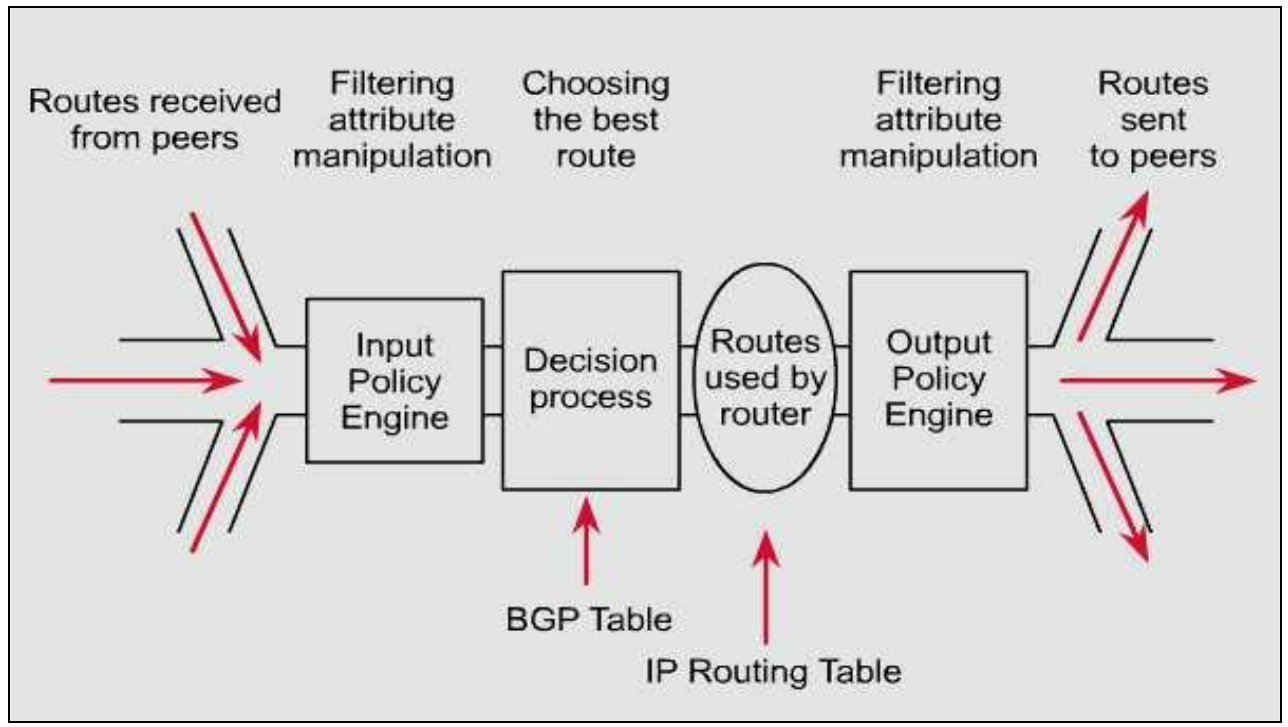
\includegraphics[scale=0.5]{../../immagini/bgp_pipe}
\end{figure}\\\\
si possono filtrare prefissi, o filtrare attributi o manipolare attributi nella fase di input policy engine.
\\Quando si decide che una rotta è la migliore si salva nel DB e si propaga agli altri vicini.
\\C'è un meccanismo molto noto che permette di influenzare la scelta del percorso, ovvero \textbf{l'AS path prepend}: le informazioni vengono cambiate includendo dei numeri di AS dummy che andrebbero ad incrementare la lunghezza del path, così da influenzare la traiettoria del traffico su una o l'atra strada. (VEDI ESEMPIO)
\\L'attributo COMMUNITY è importante, usato per controllare le topologie BGP/MPLS VPNs, è opzionale ed è come un tag: quando un vicino riceve un messaggio, può filtrare in base al valore del COMMUNITY e applicare determinate policies, andando quindi a filtrare o a modificare altri attributi.
\\Ci sono un certo numero di attributi ben noti e processati nello stesso modo dai router
\begin{itemize}
    \item NO\_EXPORT: se un router riceve una rotta con questo valore di COMMUNITY, la rotta non è esportata al di fuori dell'AS;
    \item NO\_ADVERTISE: non va inviato l'update a nessun altro;
    \item Internet: una rotta che ha questo valore, quando ricevuta, dovrebbe essere mandata a tutti gli altri
    \item Local-as: chi riceve dovrebbe inviare a tutti i peer nel suo AS ma non a quelli al di fuori di esso
    \item Custom value: il pattern dell'attributo può variare da organizzazione ad organizzazione, non serve che sia registrato e può indicare locazioni geografiche per un determinato AS mentre un advertisement per una rotta per un altro AS. 
\end{itemize}

\subsection{BGP configuration} 
Vediamo come configurare BGP su CISCO IOS, la prima cosa da fare è far girare un BGP process (QUAGGA ha la stessa sintassi dell'IOS CISCO): il comando base è \texttt{router bgp AS-number}, a differenza di OSPF un router non può far parte di diversi AS.
\\È possibile fare ri-distruzione delle rotte ai peers esterni, parliamo di milioni di entries nelle tabelle BGP quindi non è conveniente farlo per tutte le entry.
\\Si usa il comando \texttt{network} per dire al processo BGP quale rete locale va contattata, anche OSPF ha questo comando, ma ha un doppio ruolo:
\begin{itemize}
    \item si attivano i nodi sulla rete da aggiornare
    \item si connettere direttamente alla rete ad aggiornare
\end{itemize}
La cosa importante è che la rotta da voler aggiornare è già nella routing table, altrimenti l'aggiornamento si perde.
\\Il BGP peering si ottiene col comando \texttt{neighbor}, passando indirizzo IP, AS remoto e numero dell'AS.
\\Con questo comando si identifica un peer router col quale il router locale stabilirà la connessione, con l'argomento AS-number si specifica se il neighbor sarà un EBGP o IBGP.
\\Si potrebbero usare le interfacce di loopback, è utile crearla quando un peer può essere raggiunto con molteplici path, in modo da usare l'interfaccia di loopback che abbia un IP virtuale e che sia possibile da raggiungere quindi ad esempio si deve fare advertising dell'indirizzo virtuale del loopback con OSPF.

\subsection*{Lab 010}
Vediamo uno scenario BGP semplice, usiamo due tipi di loopback, usiamo i due gruppi di IP /16 nel caso di router1 per evitare di avere altre macchine collegate e per poter usare ICMP.
\\R4, R2 ed R5 possono essere raggiunti da diversi path, quindi se uno dei link fallisce è OSPF che deve ridistribuire l'informazione su come raggiungere il nodo sulla nuova rotta.
\\Fra i router di AS 200 ci sono dei link privati punto-punto, si usa OSPF anche per come raggiungere la loopback di gestione.
\\Ci sono modi per evitare che tutti i router del core debbano conoscere le tabelle di routing, se si usa una backbone MPLS, con LDP si manda in flooding a tutte le reti e si creano tutti i path MPLS per arrivare a tutti.
\\Fondamentale il discorso delle loopback: usate quando un router ha più path verso di lui perché se si può raggiungere un router, si annuncia una interfaccia virtuale e starà al protocollo di routing ottenere la strada fisica, in modo che se il link fallisce è possibile raggiungere il nodo.
\\Le loopback di management hanno /32 come subnet, le /16 sono "fittizie", in quanto simulano la presenza di una rete dietro il router.
\\OSPF conosce tutta la topologia di rete, con le aree OSPF è possibile che tutti i router interni alla stessa area condividano la stessa tabella OSPF, in modo da poter scalare meglio.
\\Tutto ciò che è fuori dalla area è visto come un indirizzo esterno, si conosce solo il router per arrivarci e non l'intera topologia.
\\Configurazione dei router CISCO, la rotta \textbf{ip route 1.0.0.0 255.0.0.0 Null0}: una best practice di BGP è compattare le entry, quindi il primo modo è compattare le entry, occorre però avere la tabella di routing per fare advertising nella sotto-rete, non manda fuori rotta per via del longest prefix matching (la /8 hanno un prefisso più lungo della /16, quindi non manda fuori rotta).
\\Tramite il comando nella configurazione BGP, si annuncia che l'indirizzo è quello della loopback interface, con next-hop-self si cambia il next hop perché di default il forwarding di un messaggio BGP con next hop interno preserva il next hop.
\\Quando si tenta il ping dal router cisco occorre dire l'indirizzo sorgente, in quanto altrimenti il ping esce con l'IP privato, non raggiungibile.

\section{MPLS}
L'idea chiave è mettere una piccola label fra il layer 2 e layer 3 ed il router che riceve il pacchetto fa solo switching e non routing: questo è il formato della label\\
\begin{figure}[h!]
    \centering
    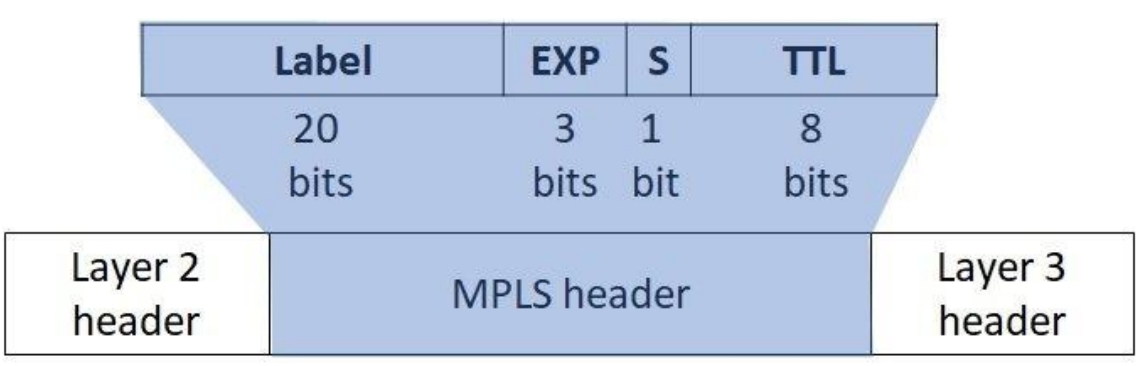
\includegraphics[scale=0.5]{../../immagini/mpls_label}
\end{figure}\\\\
il forwading in MPLS è fatto a livello 2, a livello di switching.
\\Come in molti protocolli, ci sono componente di controllo e componente di forwarding ed i due componenti sono indipendenti.
\\Prima, nel protocollo ATM c'era un campo specifico dove poter mettere la label, in Ethernet vanno aggiunti 4 byte fra livello 2 ed header IP. Terminologia:
\begin{itemize}
    \item Label Edge Router (LER): router di edge per la rete MPLS
    \item Label Switching Router: fa lo switching delle operating labels cambiando internamente la rete MPLS  
    \item Label Distribution Porotocol: congiuntamente ai protocolli di routing, LDP è usato per distribuire le label fra i device della rete
    \item Forwarding Equivalence Class (FEC): un insieme di pacchetti IP che sono forwardati nella stessa maniera, ad esempio sullo stesso percorso o con lo stesso trattamento
    \item Label Switched Path: il percorso che uno o più LSR hanno seguito per un pacchetto appartenente ad una certa FEC 
\end{itemize}

Le operazioni sono
\begin{itemize}
    \item Push: push della label di un pacchetto.
    \\LER di ingresso della backbone MPLS alaizza l'header del pacchetto IP, classifica il pacchetto e lo manda al suo LSR di next hop
    \item Forwarding: si prende la label in ingresso e si cambia con la proprio egress label.
    \\Nel cloud LSR il pacchetto viene forwardato sull LSP in accordo alla label e ad ogni hop le label vengono scambiate (label locale : label remota)
    \item Pop: il router fa pop della label e passa il pacchetto a livello IP.
    \\Siamo al LER egress, viene passato il pacchetto in base all'IP di destinazione
\end{itemize}
LDP viene usato per creare associazioni fra i LER ed i LSR, vediamo un esempio di come si distribuiscono le labels: è possibile effettuare il downstream on demand, il router che gira con LDP manderà delle label request, in modo che questi sappiano quali label porre sui pacchetti. (slides per vedere l'esempio).
\\C'è anche il tipo unsolicited, nel caso on demand si richiede esplicitamente una label per fare routing, mentre nel secondo caso si dice a tutti i neighbor di usare una certa label per raggiungere la mia rete.
\\MPLS è versatile, perché si possono stackare diverse label: se il bit di s è settato ad 1 vuol dire che non si possono aggiungere più MPLS labels, quindi dal quel punto in poi c'è un pacchetto IP.

\subsection{MPLS e BGP}
Un problema da dover affrontare in BGP è fare un full mesh delle label in modo che nessun router interno abbia informazioni sul mondo esterno e vale solo se il router non ha una rete dietro.
\\(LDP si basa sulle informazioni scambiate per i costi dei link da OSPF).
\\Nel pacchetto IP con la label MPLS c'è solo il tipo del pacchetto switchato e non di due tipi come nel caso di VLAN, perché MPLS lavora solo con IP.
\\(LAB per vedere come funziona)


\section{VPN con MPLS e BGP}
In questo caso, MPLS sarà "l'incapsulamento" e BGP il control plane di questo incapsulamento.
\\È quello che si chiama peer-to-peer VPN, che non è configurata dagli end host bensì dagli ISP: grandi compagnie che hanno diversi edifici sparsi per il mondo comprano le VPN dagli ISP per ottenere dei link con determinati QoS.
\\Per degli use case come questi, la soluzione BGP MPLS è la più usata, ha il vantaggio di essere plug\&play: se mettiamo un altro router, detto customer edge, l'IPS connette il sito alla VPN.
\\ Altra terminologia:
\begin{itemize}
    \item customer edge: il router che si interfaccia all'ISP.
    \\È il router dell'azienda con funzionalità di routing standard, il suo unico peer è il Provider edge con cui scambia informazioni mediante messaggi BGP
    \item provider edge: è l'access router dell'ISP, il primo che implementa la MPLS VPN.
    \\Sono quelli che controllano davvero i paths e che implenteranno la MPLS VPN
    \item provider router: fa il forwarding dei pacchetti basandosi sulle label, è un LSR
    \item MPLS backbone: la rete che partecipa all'MPLS vpn
\end{itemize}
Parleremo di VPN A o B etc... che è il customer con i siti sparsi in giro.
\\L'implementazione basilare: il customer edge manda un pacchetto al provider edge, che è il primo a mettere una label (il rotuer del provider non sa nemmeno che c'è una VPN) ed il control plane fornisce le label per arrivare a destinazione, avviene lo swapping al provider edge 2 che manda il pacchetto a destinazione.
\\Possiamo risolvere problemi: ad esempio, dopo la pop(), il pacchetto deve essere instradato in base alla tabella di IP del PE locale.
\\Ma se due clienti hanno gli stessi indirizzi di rete per i siti connessi alla stessa PE?
Si risolve con due label: la label esterna è il tunnel, quella interna è il customer
\begin{itemize}
    \item la label esterna identifica la VPN, che è uguale per le diverse VPN
    \item la label interna può essere cambiata
    \item nell'ultimo edge provider abbiamo la label interna, rimossa la esterna, in base a questa si decide dove forwardare il pacchetto
\end{itemize}

\subsection{Gestione della VPN}
Occorre gestire diverse forwarding table, possiamo avere tante VPN e routing table quanti i client connessi ad un certo device, la tabella di forwarding MPLS cambia in base alla specifica VPN a cui appartiene il cliente.
\\Il PE deve supportare tante tabelle di forwarding quanti sono i clienti connessi alla VPN e tali tabelle sono anche dette VPN Routing and Forwarding tables (VRF).
\\Nel VRF si inserisce il VPN network address da raggiungere, la maschera, l'IP del prossimo provider edge.
\\Oltre questo, il PE salva anche le Global Forwarding Table (GRT) che permettono di raggiungere il PE da un altro PE.
\\Ogni entry della GRT contiene le tuple con IP del PE, label esterna, interfaccia di output.
\\Le GTF vengono popolate dal provider nel momento in cui avviene il setup della VPN, quindi è popolata automaticamente da LDP.
\\La VRF contiene due categorie di forwarding:
\begin{itemize}
    \item forwarding a siti LOCALI
    \item forwarding a siti REMOTI
\end{itemize}
le informazioni sul forwarding locale possono essere configurate a mano o ottenute mediante un protocollo di routing specifico (OSPF, RIP etc...), mentre le rotte remote tramite un estensione del protocollo BGP detto MP-IBGP, è BGP semplice ma negli announcments si possono mettere più informazioni, quindi gli annunci conterranno le informazioni sulle VPN e ci sono le stesse regole di BGP, quindi avremo un overlay full mesh fra tutti i provider edges.
\\Viene fatta l'assunzione che il costo di un salto diretto fra due hop PEs è 1, dato che è un salto a livello IP.
\\Grazie agli annunci MP-iBGP, l'engine BGP nei PE può calcolare i next hop verso ogni prefisso annunciato.
\\Inoltre le VRF appartenenti a diverse VPN possono notificare uno stesso prefisso privato visto che è possibile gestire overlap fra gli spazi degli indirizzi. 
\\L'identificatore più importante della MP-iBGP è il \textbf{route distinguisher}, che è unico per la VPN ma può essere usato anche dagli altri provider edges ed è best practice che ogni customer abbia un route distinguisher unico, viene messo prima dell'indirizzo nell'annuncio BGP.\\
(Esempio sulle slides per come si popola la VRF).
Il route distinguisher è cosa distingue la VPN da una customer VPN, in quanto viene messo prima della rete all'interno del messaggio, nel pacchetto ci sono anche le label interne ed esterne dove l'esterna identifica il tunnel mentre l'interna la VPN.
\\Nella topologia VPN, in iBGP c'è una full mesh fra tutti i nodi chge partecipano all'iBGP ma il problema è che se le rotte vengono scambiate usando iBGP tutti si connettono con tutti e ci son use case in cui si vuole invece avere ad esempio una topologia hub\&spoke.
\\Per cambiare la topologia di una certa VPN, occorrerebbe cambiare tutto l'MP-iBGP overlay, quindi la scelta è quella che ogni proveider edge decide quali annunci accettare dagli altri provider edges: se ad esempio tutti i provider accettano tutti gli adv, abbiamo questo risultato:\\
\begin{figure}[h!]
    \centering
    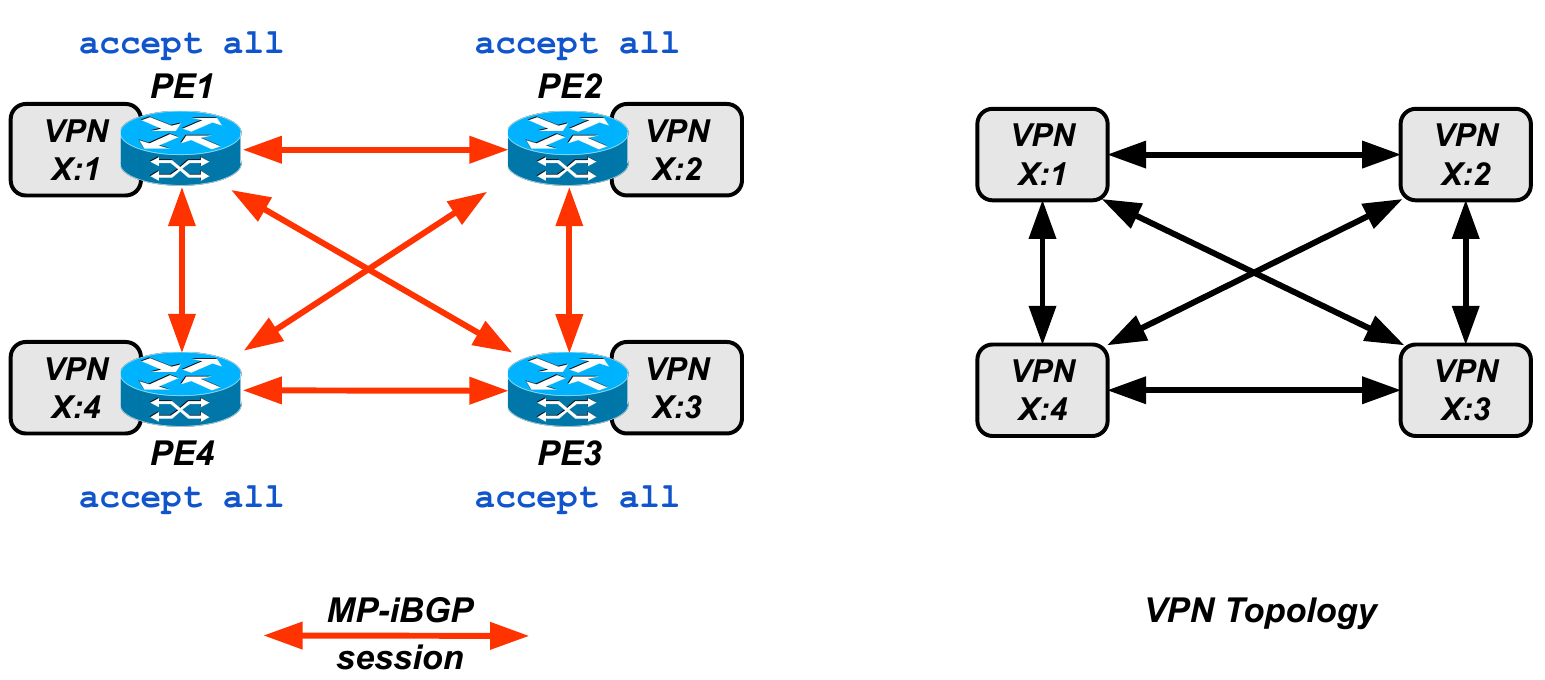
\includegraphics[scale=0.5]{../../immagini/vpn_fullmesh}
\end{figure}\\\\
se invece vogliamo una topologia di tipo h\&s, abbiamo questo tipo di risultato:\\
\begin{figure}[h!]
    \centering
    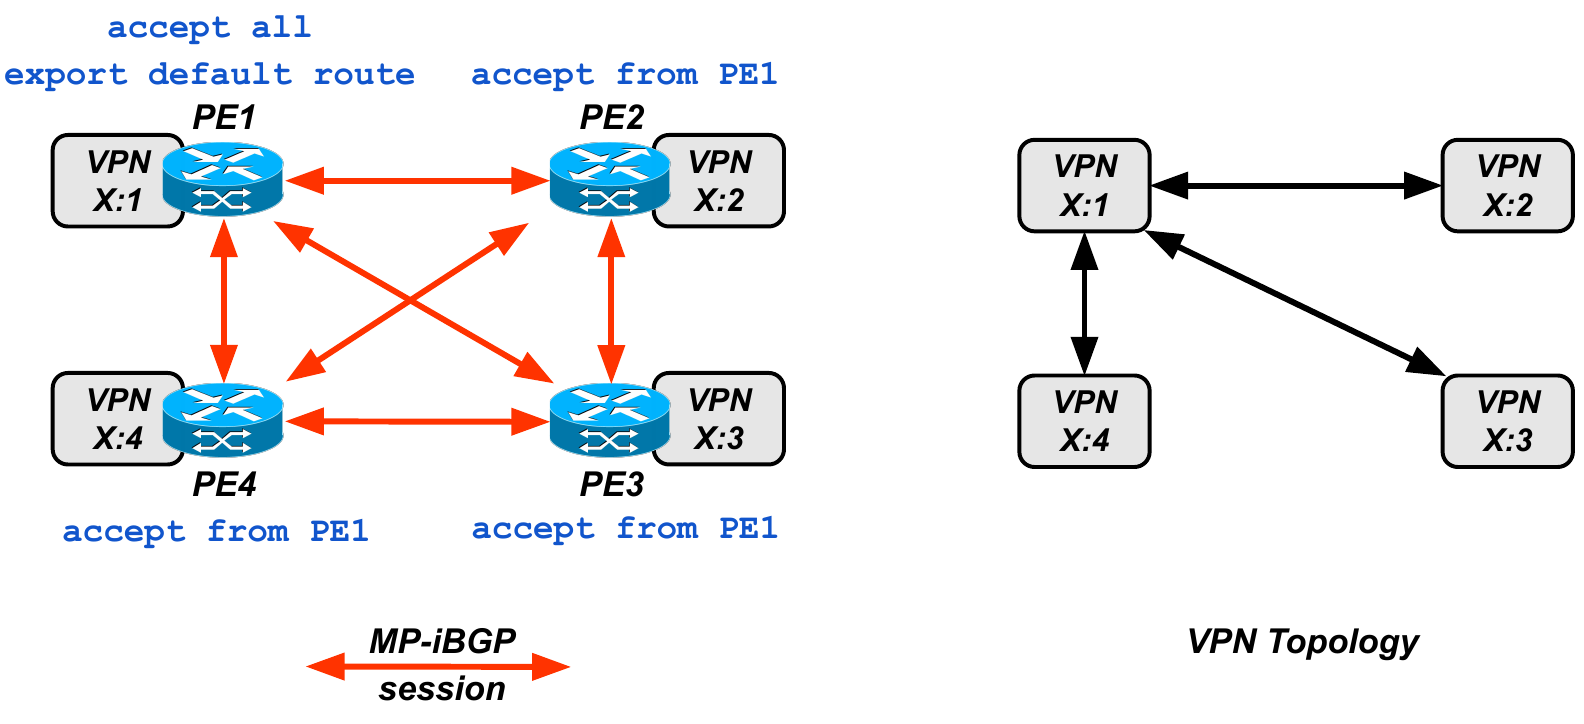
\includegraphics[scale=0.5]{../../immagini/vpn_hs}
\end{figure}
ad esempio, il provider edge 3 esporterà una certa rotta ed in questo caso pe1 accetta mentre pe2 rifiuta la rotta.
\\Possiamo quindi avere situazioni di mesh parziale, per farlo si usa un altro identificatore che è il \textbf{route target}: è configurabile, di 64 bit e ciò che si fa è configurare quali id si vuole esportare ed importare, il modo di definire i 64 bit in BGP è 32:32.
\end{document}
